\documentclass[12pt]{article}
\usepackage{amsmath}
\usepackage{fontspec}
\usepackage{xunicode}
\usepackage{xltxtra}
\setromanfont{FreeSerif}
\setsansfont{FreeSans}
\setmonofont{FreeMono}
\usepackage{caption}
\usepackage{subcaption}


\usepackage{geometry}
 \geometry{
 a4paper,
 total={210mm,297mm},
 left=20mm,
 right=20mm,
 top=20mm,
 bottom=20mm,
 }
 \usepackage{graphicx}
 \DeclareGraphicsExtensions{.pdf,.png,.jpg}
\usepackage{float}

\title{Groceries}
\author{Ευάγγελος Καραγεώργος - Βασίλιος Σκούρτης }
\date{}
\begin{document}
  \maketitle
  \section{Περιγραφή}
  	\paragraph{}
  	  Η εργασία είναι ένα λειτουργικό e-shop, που εμπορεύεται τρόφιμα και άλλα είδη παντοπωλείου. Το site υλοποιήθηκε σε PHP χωρίς να χρησιμοποιηθεί κάποιο framework, ως σκέτος PHP κώδικας για server-side κώδικα σε συνδιασμό με javascript με τη χρήση JQuery και JQueryUI βιβλιοθήκες και απλό CSS για τον client-side κώδικα και styling. Η βάση είναι υλοποιημένη σε MySql και χρησιμοποιήται το πακέτο WAMP για Apache, PHP και MySql διανομή της εφαρμογής.
  	  \par Το κατάστημα έχει προϊόντα χωρισμένα σε ομάδες, χρήστες που είναι απλοί πελάτες ή διαχειριστές, καλάθια επισκεπτών, και παραγγελίες. Η ροή της παραγγελίας είναι ως εξής:
  	  \begin{enumerate}
  	  	\item Προσθήκη προϊόντων στο καλάθι.
  	  	\item Προβολή της σελίδας του καλαθιού και μεταβολές σ'αυτο.
  	  	\item Καταχωρηση παραγγελίας. Ο χρήστης θα πρέπει να εισάγει αριθμό πιστωτικής, να συμφωνησει με τους όρους του καταστήματος και να υποβάλει επιτυχώς την παραγγελία. Κατά την υποβολή της παραγγελίας θα του εμφανιστεί η σελίδα απόδειξης. Η παραγγελία θα δημιουργηθει ως έγκυρη και θεωρείται εν'εξελίξει.
  	  	\item Επιβεβαίωση απο διαχειριστή. Ενας διαχειριστής, εφόσον επιβεβαιώσει τραπεζικώς την πληρωμή, είτε θα ακυρώσει την παραγγελία, είτε θα την ολοκληρώσει.
  	  \end{enumerate}
  	  \par Οι επισκέπτες έχουν τη δυνατότητα να πλοηγηθούν στα προιόντα και διαχειριστούν το καλάθι τους. Οι συνδεδεμένοι χρήστες έχουν επιπλέον τη δυνατότητα να υποβάλλουν παραγγελίες και να μπούν στις σελίδες διαχείρισης λογαριασμού. Οι διαχειριστές μπορούν εκτός απο τα παραπάνω, να δουν στατιστικά του καταστήματος, να επιβεβαιώσουν παραγγελίες και να προμη-θεύσουν τα προιόντα που τελειώνει το stock τους.
  \section{Βάση}
  	\subsection{E-R διάγραμμα}
		\begin{figure}[H]
			\centering
			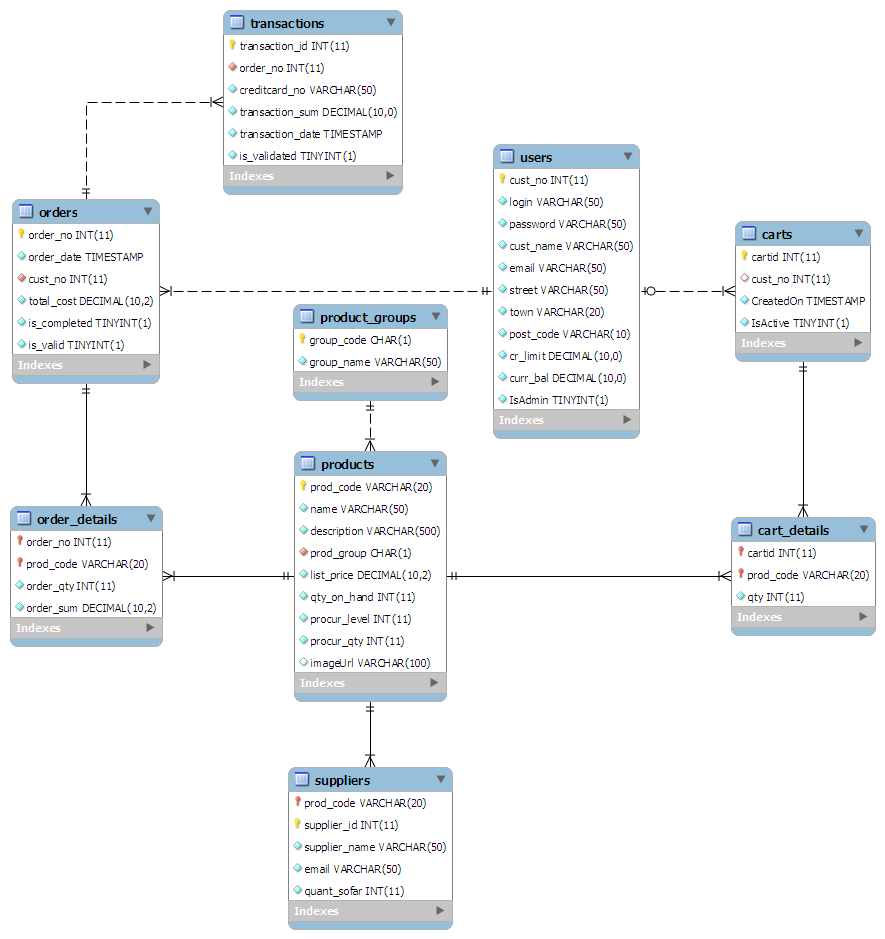
\includegraphics[width=1\textwidth]{ER_model}
			\caption{Groceries E-R model}
		\end{figure}
	\pagebreak
	\subsection{Functions και Procedures}
  	  \paragraph{}
  	  	Πολλές από τις βασικές λειτουργίες υλοποιούνται με τη βοήθεια κάποιων functions και procedures που φροντίζουν πολλές λειτουργίες να γίνονται atomic και με ασφάλεια:
  	  	\begin{itemize}
  	  		\item procedure user\_login (ilogin, ipassword) : Λαμβάνοντας ένα login name και ένα password, η διαδικασία ελέγχει τα στοιχεία και κάνει ενα select επιστρέφοντας ένα table με IsAuth, IsAdmin και cust\_no, που υποδηλώνουν εάν τα στοιχεία αντιστοιχούν σε χρήστη, εάν ο χρήστης είναι admin και ποιό είναι το cust\_no του χρήστη (-1 στην περίπτωση που τα στοιχεία είναι λάθος).
  	  		\item function user\_register (ilogin, ipass, ifullname, iemail, istreet, itown, ipostcode) : Εγγράφει έναν νέο χρήστη εάν το login name δεν υπάρχει ήδη. Επιστρέφει το cust\_no του χρήστη που προστέθηκε, αλλιώς -1.
  	  		\item function add\_to\_cart (icartid, iprod\_code, iqty) : Προσπαθεί να προσθέσει στο καλάθι με cartid = icartid, ποσότητα iqty από το προιόν με κωδικό iprod\_code. Η ποσότητα που προσθέτουμε μπορεί να είναι και αρνητική για να αφαιρέσουμε από το καλάθι. Η συνάρτηση ελέγχει και το stock του προϊόντος και κάνει τις απαραίτητες ρυθμίσεις, ώστε να είναι συμβατή η τελική ποσότητα με το qty\_on\_hand του προιόντος. Επίσης, εάν το προϊόν καταλήξει να είναι με ποσότητα 0, αφαιρείται απ'τον πίνακα cart\_details εντελώς. Η συνάρτηση επιστρέφει την τελική διαφορά ποσότητας σε σχέση με την προηγούμενη ποσότητα που είχε το προϊόν.
  	  		\item procedure get\_cart (icartid) : Η διαδικασία κανονικοποιεί ολόκληρο το καλάθι με cartid-icartid, όσον αφορά τις ποσότητες των προϊόντων και το qty\_on\_hand τους, πιθανόν και αφαιρώντας αυτά που δεν έχουν stock καθόλου, και κάνει ένα select με όλα τα δεδομένα του καλαθιού.
  	  		\item function convert\_cart\_to\_order (icartid) : Μετατρέπει ένακαλάθι σε παρραγελία. Εάν το καλάθι δεν υπάρχει ή είναι ανενεργό ή ο χρήστης που αντιστοιχεί στο καλάθι δεν έχει αρκετό cr\_limit-curr\_bal για να χρεωθεί την παραγγελία, η συνάρτηση επιστρέφει αρνητικό αριθμό που αντιστοιχεί στην αποτυχία. Αλλιώς, η συνάρτηση κάνει normalize το καλάθι, φτιάχνει μία παραγγελία, την ορίζει να περιέχει τα περιεχόμενα του καλαθιού, ορίζει το καλάθι ως ανενεργό, προσθέτει στο curr\_bal του χρήστη το ποσό της παραγγελίας, αφαιρεί τις΅ποσότητες των προϊόντων απο το qty\_on\_hand τους και επιστρέφει τον αριθμό παραγγελίας που δημιουργήθηκε.
  	  		\item procedure create\_transaction (iorder\_no, icretidcard\_no) : Δημιουργεί μία συναλλαγή πληρωμής για μία παραγγελία με έναν συγκεκριμένο αριθμό πιστωτικής κάρτας. Το ποσό συναλλαγής ορίζεται αυτό του κόστους της παραγγελίας.
  	  		\item procedure cancel\_order (iorder\_no) : Ακυρώνει μία εν'εξελίξει παραγγελία με το να την ορίζει ως΅άκυρη και να επιστρέφει τις ποσότητες των προϊόντων στα αντίστοιχα qty\_on\_hand.
  	  		\item function complete\_order (iorder\_no) : Εφόσον ελέγξει ότι η παραγγελία υπάρχει, είναι εν'εξελίξει και υπάρχει το αντίστοιχο transaction με το ποσό, ορίζει την παραγγελία ως ολοκληρωμένη και επιστρέφει 1. Σε περίπτωση αποτυχίας επιστρέφει 0.
  	  		\item function supply\_produc\_new\_supplier (iprod\_code, isuppliername, isupplieremail) : Εάν το όνομα προμηθευτή υπάρχει ήδη επιστρέφει -1, αλλίώς δημιουργεί νέο προμηθευτή με τα στοιχεία για το προϊόν (και το σωστό quant\_sofar ανάλογαα με το procur\_qty), πεοσθέτει στο qty\_on\_hand to procur\_qty του προϊόντος και επιστρέφει το supplier\_id που δημιουργήθηκε.
  	  		\item procedure supply\_product (iprod\_code, isupplier\_id) : Προμηθεύει το προϊόν από τον συγκεκριμένο προμηθευτή κάνοντας τα κατάλληλα adjustments σε qty\_on\_hand, quant\_sofar και προσθέτοντας την κατάλληλη εγγραφή στον πίνακα suppliers εάν δεν υπάρχει ήδη.
  	  	\end{itemize}
  	\subsection{Queries}
  	  \paragraph{}
  	  	 Τα βασικά και πιο αντιπροσωπευτικά queries που λαμβάνουν χώρα στη βάση είναι τα εξής:
  	  	 \begin{itemize}
  	  	 \item Τα γενικά queries όπου χρησιμοποιούνται για την παρουσίαση του περιέχομενου του eshop και κατά κύριο λόγο φιλτράρουν την πληροφορία βάσει των αναγκών του πελάτη.
  	  	 \item Να σημειωθεί ότι τα γενικά queries είναι διαθέσιμα σε public οθόνες, ενώ λαμβάνουν ως εισόδους αρκετές παραμέτρους.
  	  	 \item Τα προσωπικά queries, τα οποία χρησιμοποιούνται στις protected σελίδες λογαριασμών, όπου χρησιμοποιούνται από τον εκάστοτε χρήστη για να ενημερωθεί για τις προσωπικές του κινήσεις.
  	  	 \item Τα στατιστικά queries, τα οποία είναι διαθέσιμα μόνο στην admin area και παρέχουν πληροφορία στον admin για το σύνολο της εφαρμογής.
  	  	 Σε αυτές τις οθόνες, ο χρήστης μπορεί να επιλέξει το πλήθος των αποτελεσμάτων καθώς και την περίοδο που θέλει να εξετάσει.
  	  	 \end{itemize}
  	  	 
  	  	 
  	  \paragraph{}
  	  	 Στη βασική οθόνη αναζήτησης, υπάρχουν 3 κατηγορίες φιλτραρίσματος οι οποίες ενεργούν συζευκτικά.
  	  	 Αναζήτηση με κείμενο, λέξεις κλειδιά και search τύπου LIKE, με επιλογή κατηγοριών, οι οποίες είναι ΙΝ(σετ) και Price Range.
  	  	 Επίσης, ο χρήστης έχει τη δυνατότητα για διάταξη των αποτελεσμάτων βάσει του πεδίου της επιλογής του.
  	  	 
		\begin{figure}[H]
			\centering
			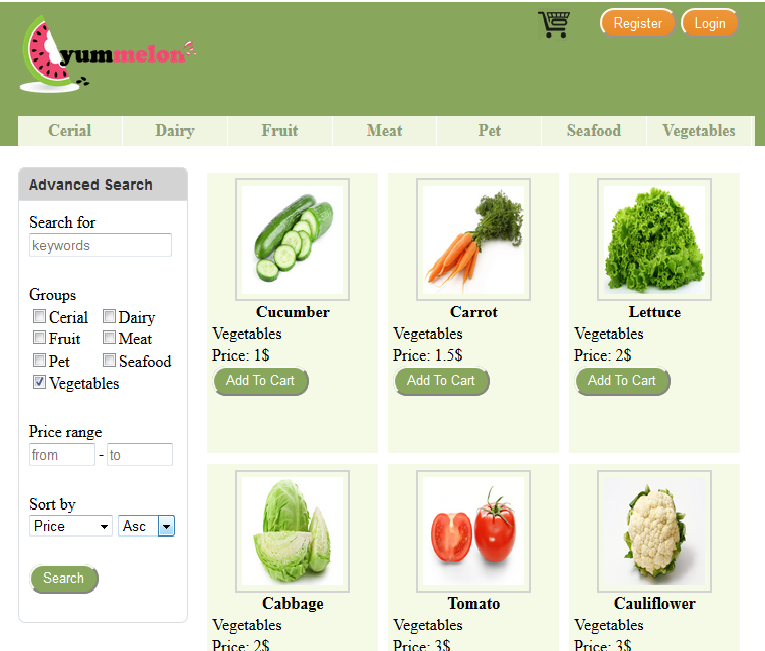
\includegraphics[width=1\textwidth]{searchImages}
			\caption{Αναζήτηση προϊόντων}
		\end{figure}
  	  	 
  	  \paragraph{}
  	  	 Το χαρακτηριστικότερο παράδειγμα προσωπικών queries αποτελούν οι παραγγελίες του χρήστη και οι λεπτομέρειες αυτών.
  	  	 
		\begin{figure}[H]
			\centering
			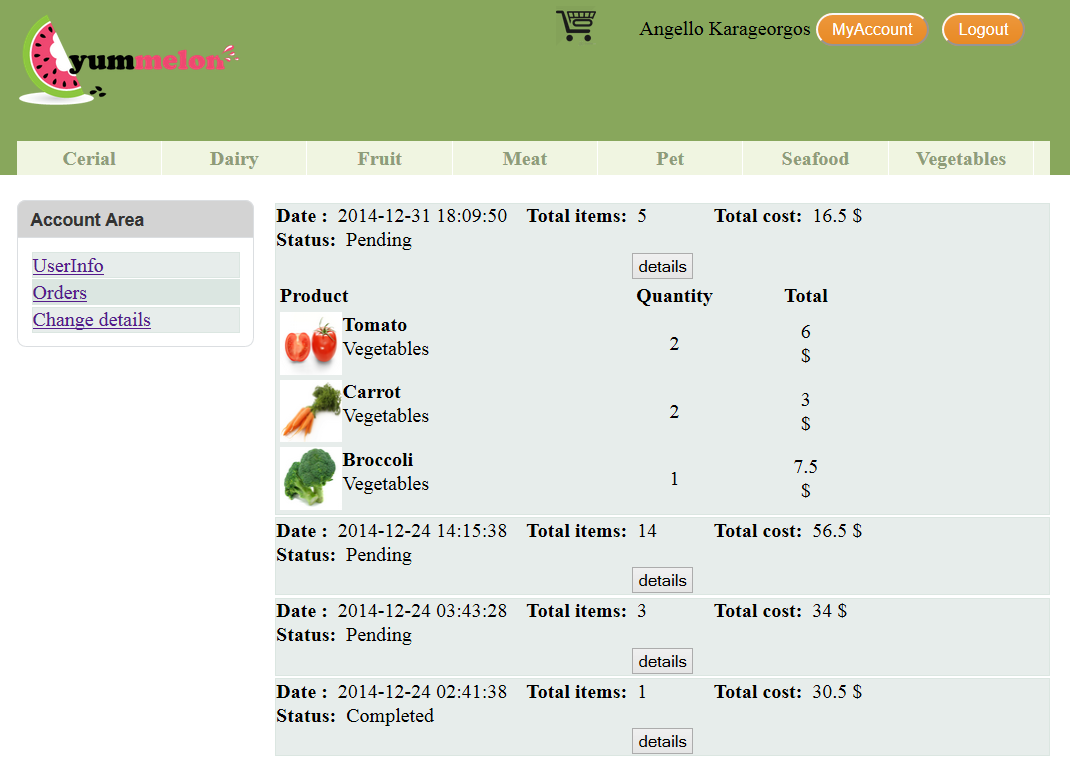
\includegraphics[width=1\textwidth]{userOrders}
			\caption{Παραγγελίες χρήστη}
		\end{figure}
  	  	 
  	  \paragraph{}
  	  	 Τέλος, ένα πλήθος οθονών και στατιστικών queries βρίσκονται στην admin area.
  	  	 Παρουσιάζονται τρείς εξ'αυτών.

		\begin{figure}[H]
			\centering
			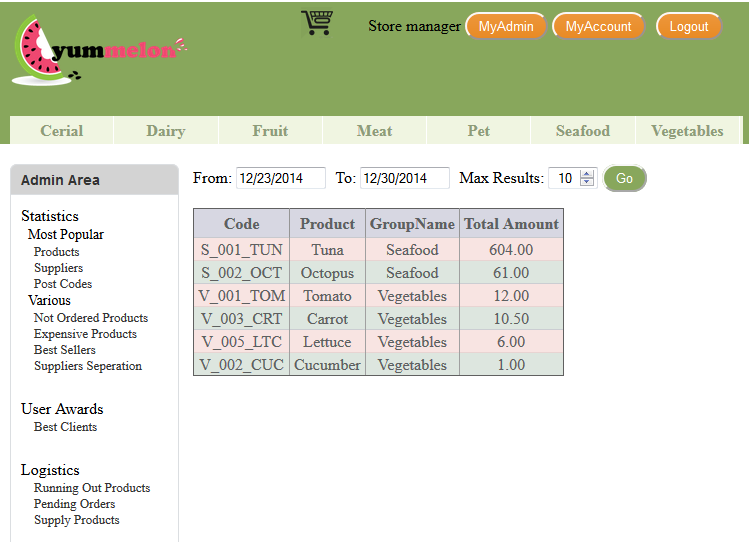
\includegraphics[width=1\textwidth]{adminArea}
			\caption{Best sellers}
		\end{figure}
		\begin{figure}[H]
			\centering
			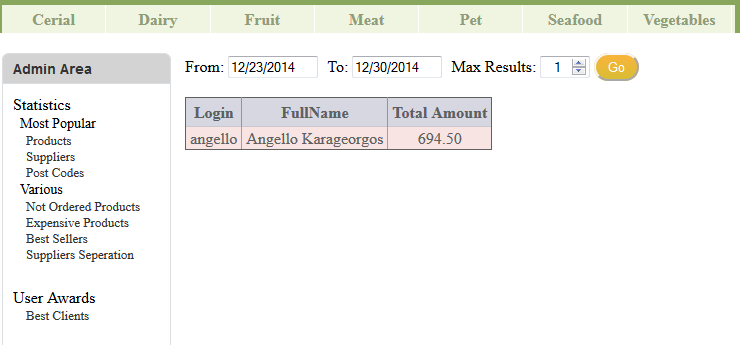
\includegraphics[width=1\textwidth]{topCustomers}
			\caption{Καλύτεροι πελάτες}
		\end{figure}  	
		\begin{figure}[H]
			\centering
			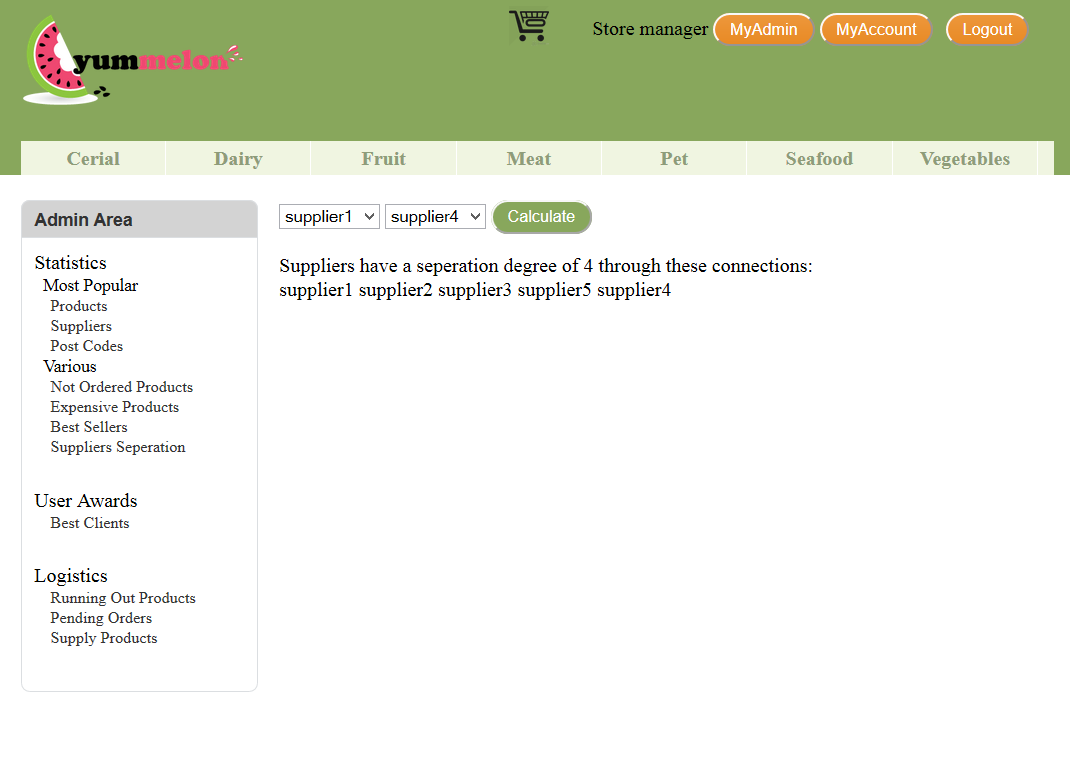
\includegraphics[width=1\textwidth]{suppliersSeperation}
			\caption{Suppliers seperation}
		\end{figure} 
	\section{Χρήστες}
	  \paragraph{}
		Οι χρήστες χωρίζονται σε 2 κατηγορίες, τους κανονικούς πελάτες-χρήστες και τους χρήστες με διαχειριστικά δικαιώματα. Για το λόγο αυτό προστέθηκε και το πεδίο isAdmin στον πίνακα users.
	  \paragraph{}
		Επίσης, οι οθόνες χωρίζονται σε 3 είδη, σύμφωνα με το ποιοι μπορούν να τις επισκεφθούν. Εχουμε τις public, τις protected και τις admin.
		\begin{itemize}
	  	  \item Τις public μπορούν να τις επισκεφθούν και προσπελάσουν όλοι.
	  	  \item Τις protected μόνο όσοι είναι εγγεγραμμένοι στο σύστημα, έχουν γίνει δηλαδή registered, και έχουν κάνει login.
	  	  \item Τις admin μόνο όσοι έχουν συνδεθεί και έχουν τον αντίστοιχο ρόλο.
		\end{itemize}
	
		\begin{figure}[H]
			\centering
			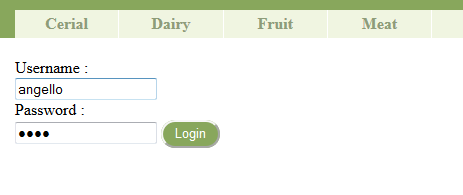
\includegraphics[width=1\textwidth]{login}
			\caption{Είσοδος χρήστη}
		\end{figure}
		\begin{figure}[H]
			\centering
			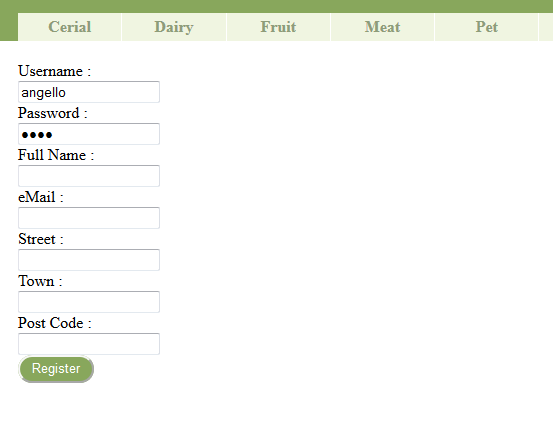
\includegraphics[width=1\textwidth]{register}
			\caption{Εγγραφή νέου χρήστη}
		\end{figure}

		
		\paragraph{}
		
		  Οι απλοί χρήστες έχουν τη δυνατότητα να προσπελάσουν το λογαριασμό τους από την επιλογή MyAccount.

		\begin{figure}[H]
			\centering
			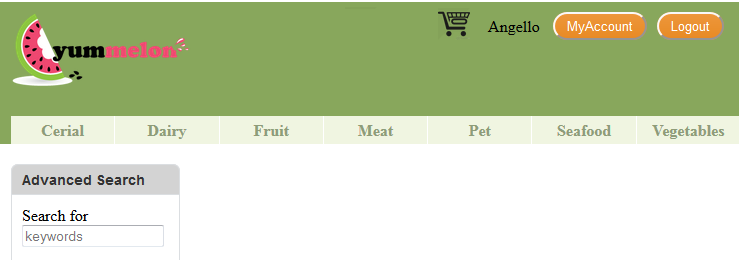
\includegraphics[width=1\textwidth]{customer}
			\caption{Σύνδεσμος για την οθόνη διαχείρισης λογαριασμού}
		\end{figure}
		
		
		\paragraph{}
		  Ο admin user πέρα από το λογαριασμό του, έχει επιπλέον τη δυνατότητα να προσπελάσει την Admin area, όπου μπορεί να πραγματοποίησει διαφορες διαχειριστικες ενέργειες καθώς και στατιστικά queries.
		  
		  Ο Admin μεταφέρεται στην admin area από την επιλογή MyAdmin.
		\begin{figure}[H]
			\centering
			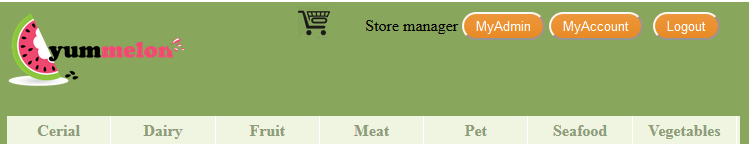
\includegraphics[width=1\textwidth]{admin}
			\caption{Σύνδεσμος για την admin area}
		\end{figure}
	\section{Λειτουργίες}
	  \subsection{Επισκέπτες}
	  	 \paragraph{}
	  	 	Οι επισκέπτες μπορούν να ψάχνουν τα προϊόντα μέσω της αναζήτησης προϊόντων και να βλέπουν λεπτομέρειες του κάθε προϊόντος απ'τη σελίδα λεπτομερειών προϊόντος.
			\begin{figure}[H]
				\centering
				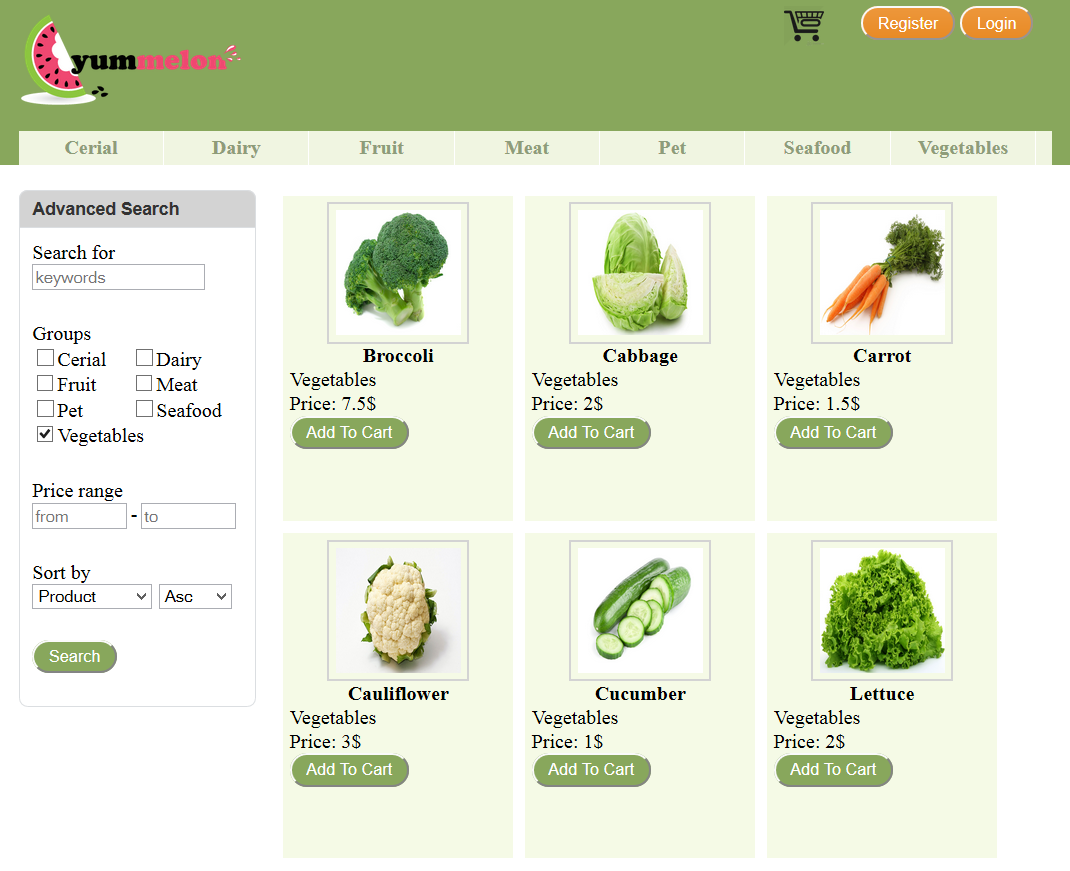
\includegraphics[width=1\textwidth]{productList}
				\caption{Λίστα προϊόντων}
			\end{figure}
			\begin{figure}[H]
				\centering
				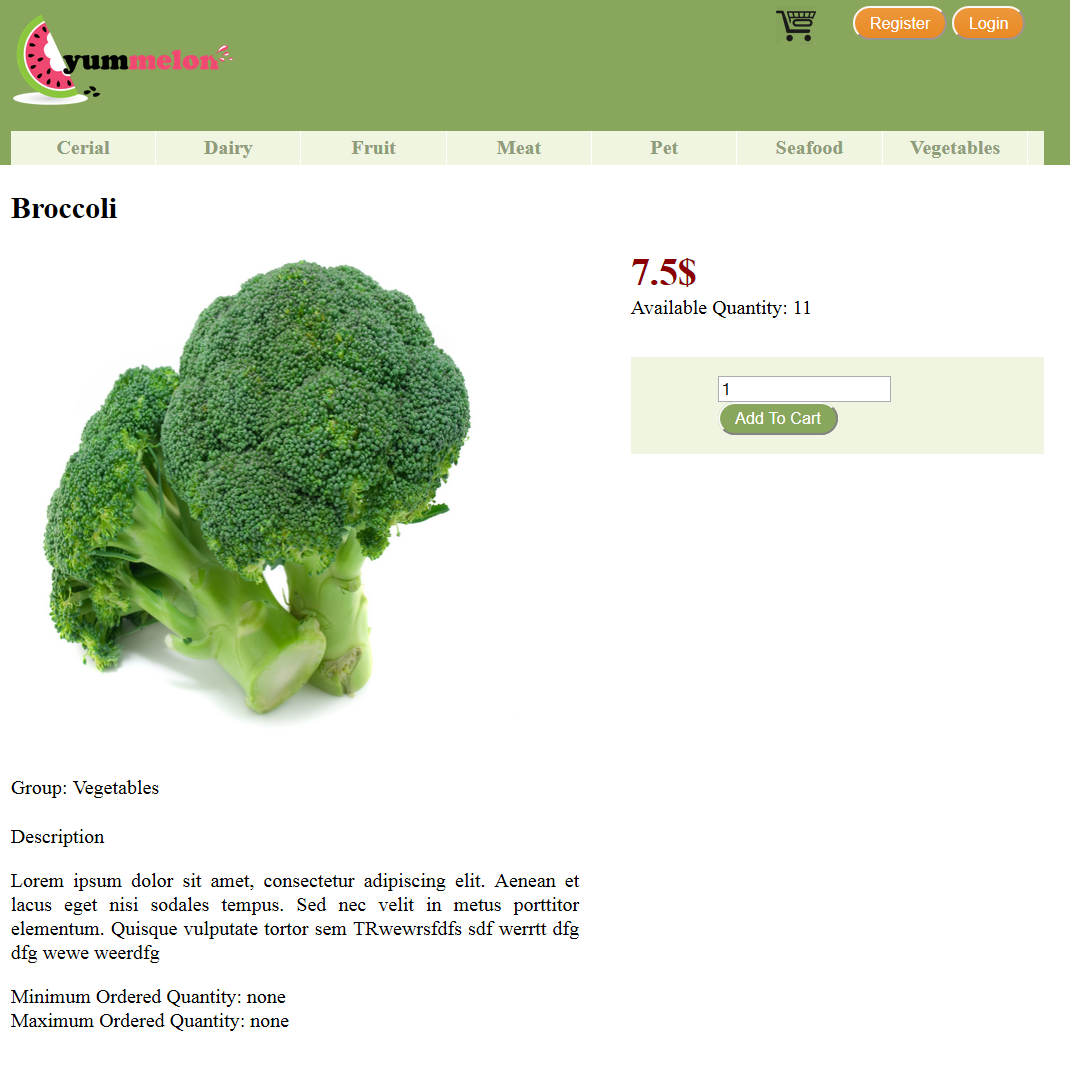
\includegraphics[width=1\textwidth]{productDetails}
				\caption{Λεπτομέρειες προιόντος}
			\end{figure}	  
		  \paragraph{}
			Στη λίστα προϊόντων ή στις λεπτομέρειες προϊόντος υπάρχει το κουμπι για προσθήκη στο καλάθι. Πατώντας αυτό το κουμπί, το προϊόν προστίθεται στο καλάθι του επισκέπτη, η εάν δεν υπάρχει απόθεμα, εμφανλιζεται μύνημα λάθους κατάλληλο. Ο επισκέπτης, μπορεί να μπεί στη σελίδα του καλαθιού, οπού εμφανίζονται τα προϊόντα που έχει προσθέσει στο καλάθι, μαζί με τις ποσότητές τους και υπάρχει η δυνατότητα να κάνει οτιδήποτε αλλαγές στο καλάθι. 	
			\begin{figure}[H]
				\centering
				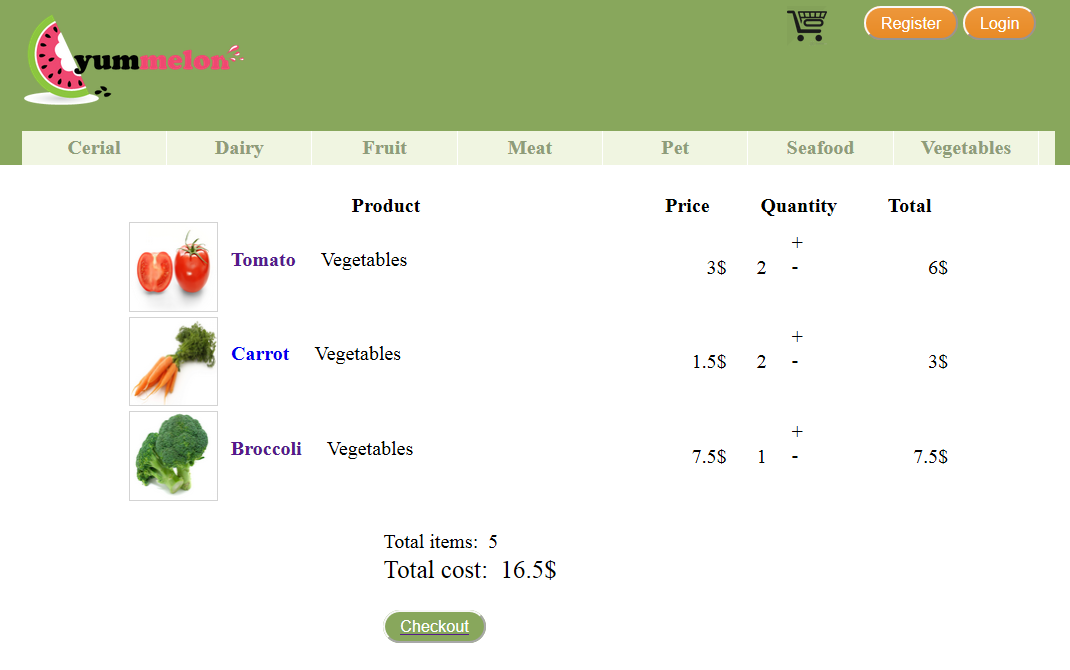
\includegraphics[width=1\textwidth]{cart}
				\caption{Καλάθι επισκέπτη}
			\end{figure}
		  \paragraph{}
			Εάν ο επισκέπτης πατήσει στη σελίδα του καλαθιού το κουμπί "checkout", μεταφέρεται στη σελίδα ολοκλήρωσης παραγγελίας. Οι επόμενες σελίδες είναι προστατευμένες, συνεπώς ο επισκέπτης θα κληθεί να κάνει login για να προχωρήσει, εάν δεν είναι ήδη συνδεδεμένος. Στη σελίδα υποβολής της παραγγελίας θα παρουσιαστούν τα προϊόντα προς παραγγελία, ένα πεδίο να συμπληρωθεί ο αριθμός πιστωτικής και ένα checkbox που θα πρέπει να πατηθεί, που δηλώνει ότι ο χρήστης΅συμφωνεί με τους όρους παραγγελίας του καταστήματος.
			\begin{figure}[H]
				\centering
				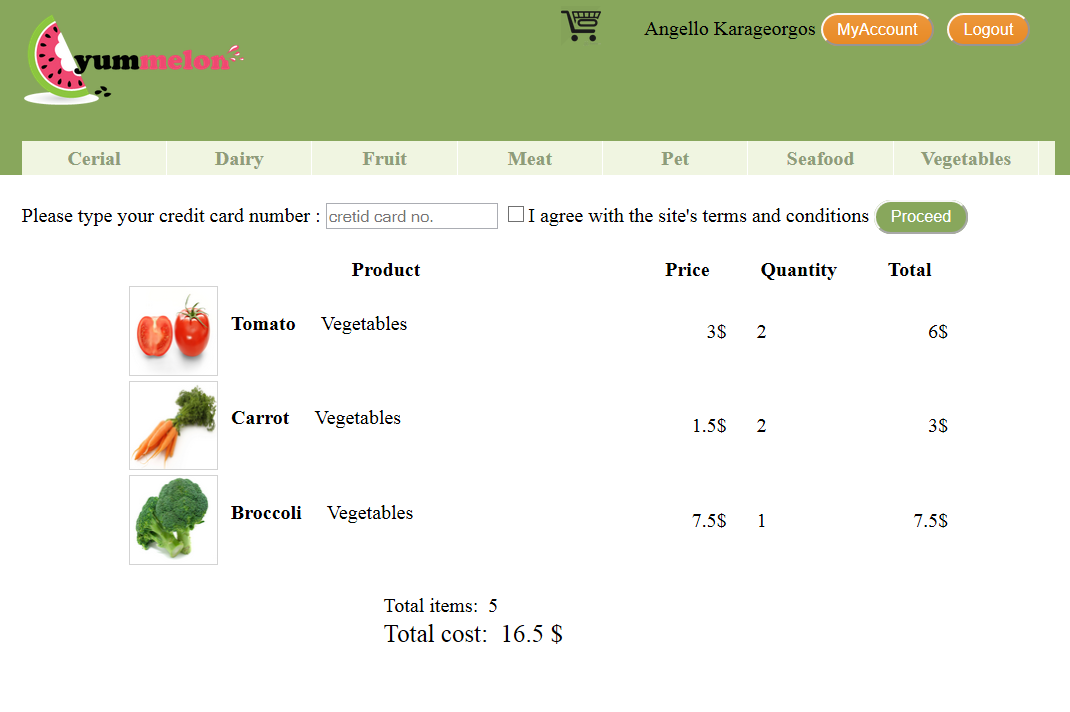
\includegraphics[width=1\textwidth]{checkout}
				\caption{Υποβολή παραγγελίας}
			\end{figure}
		  \paragraph{}
			Εάν ο χρήστης εισάγει αριθμό πιστωτικής και πατήσει το checkbox, μπορεί να πατίσει το κουμπί "proceed" για να καταχωρήσει την παραγγελία. Εάν η καταχώρηση γίνει επιτυχώς, θα μεταφερθεί στην σελίδα επιβεβαίωσης της παραγγελίας, όπου έχει τη μορφή απόδειξης.
			\begin{figure}[H]
				\centering
				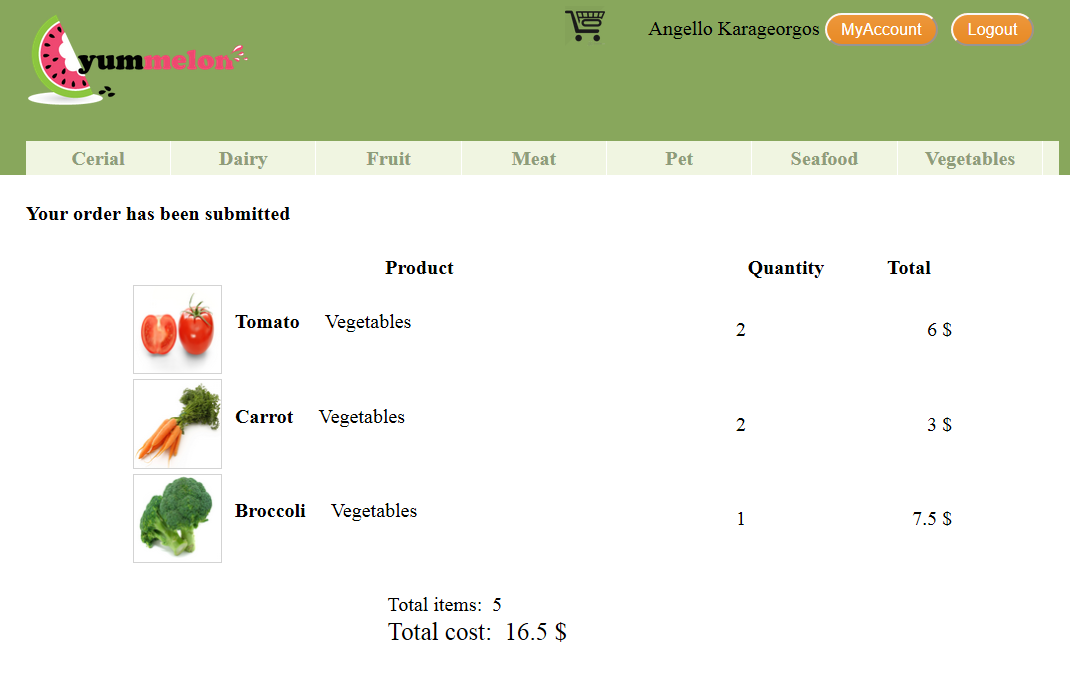
\includegraphics[width=1\textwidth]{invoice}
				\caption{Απόδειξη παραγγελίας}
			\end{figure}

	  \subsection{Χρήστες}
	  	 \paragraph{}
	  	 	Οι συνδεδεμένοι χρήστες, εκτός της απλής πλοήγησης και της δημιουργίας και υποβολής παραγγελιών, μπορούν να μοπύν στις account σελίδες μέσω του συνδέσμου "MyAccount" στην κορυφή της κάθε σελίδας. Οι account σελίδες είναι οι εξής:
	  	 	\begin{itemize}
	  	 	  \item UserInfo : Η αρχική σελίδα, που εμφανίζει τις πληροφορίες του χρήστη.
	  	 	  \item Orders : Η σελίδα που προβάλλει τις παραγγελίες που έχει υποβάλλει ο χρήστης, μαζί με τις λεπτομέρειές τους και την κατάστασή τους.
	  	 	  \item Change details : Η σελίδα που μπορείς να αλλάξεις τα στοιχεία του χρήστη.
	  	 	\end{itemize}
			\begin{figure}[H]
				\centering
				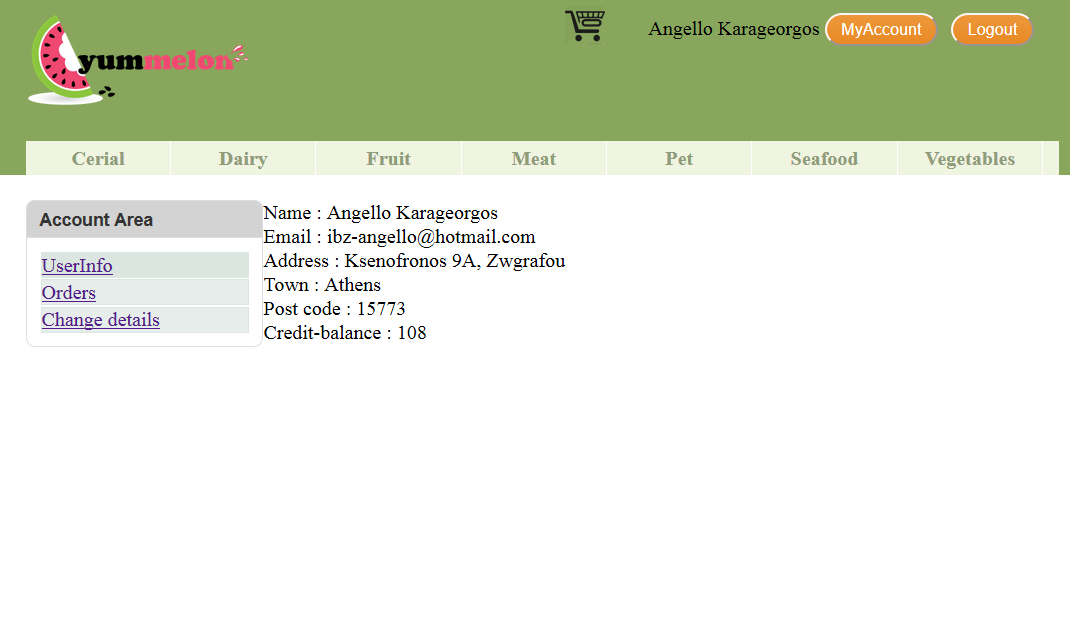
\includegraphics[width=1\textwidth]{userInfo}
				\caption{UserInfo}
			\end{figure}
			\begin{figure}[H]
				\centering
				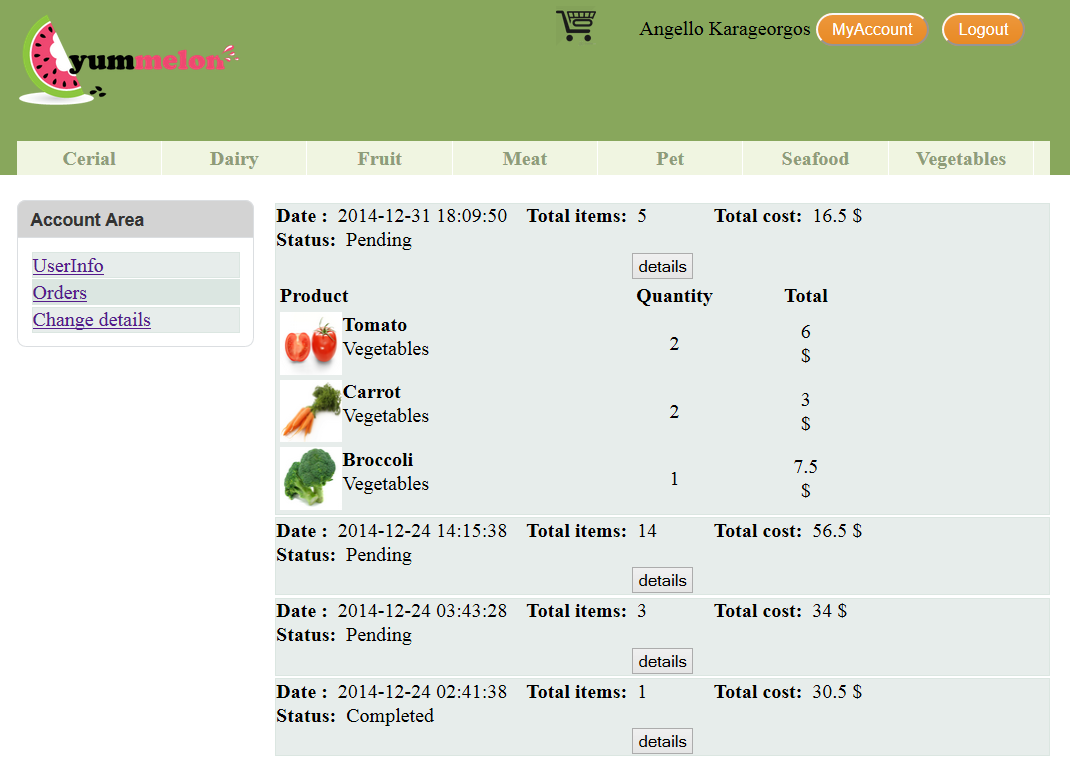
\includegraphics[width=1\textwidth]{userOrders}
				\caption{Orders}
			\end{figure}
			\begin{figure}[H]
				\centering
				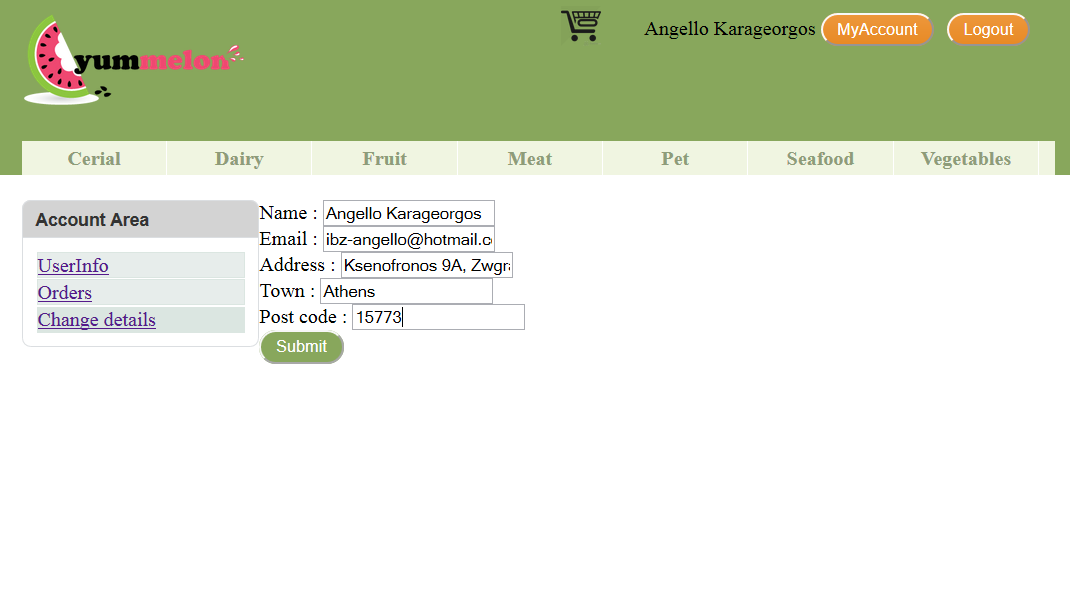
\includegraphics[width=1\textwidth]{userChangeInfo}
				\caption{Change details}
			\end{figure}	  

	  \subsection{Διαχειριστές}
	  	 \paragraph{}
	  	 	Ενας διαχειριστής, εκτός απο τις λειτουργίες που μπορεί ν κάνει οποιοσδήποτε χρήστης, μπορεί να μπει και στισ admin σελίδες. Στις admin σελίδες΅, εκτός απο τα βασικά queries που μπορούν να προβληθούν, όπως τους καλύτερους πελάτες, τα best seller προιόντα κλπ., ο διαχειρηστής μπορεί να κάνει και επιπλέον λειτουργίες του καταστήματος:
	  	 	\begin{itemize}
	  	 	  \item Pending orders : Η προβολή μη-ολοκληρωμένων παραγγελιών, που έχουν υποβληθεί απο πελάτες΅, αλλά δεν έχουν επιβεβαιωθεί ακόμη. Ο διαχειριστής μπορεί κάθε εν'εξελίξη παραγγελία να την ολοκληρώσει ή να την ακυρώσει.
	  	 	  \item Supply products : Η σελίδα προμήθευσης των προϊόντων. Ο διαχειριστής βλέπει ποιά προιόντα έχουν stock κάτω απο το επίπεδο που έχει οριστεί στη βάση ως procur\_level και μπορεί να εκτελέσει την προμήθειά τους΅από έναν από τους υπάρχοντες προμηθευτές ή κάποιον καινούριο με τα κουμπιά "supply" και "Add supplier" αντίστοιχα.
	  	 	\end{itemize}
			\begin{figure}[H]
				\centering
				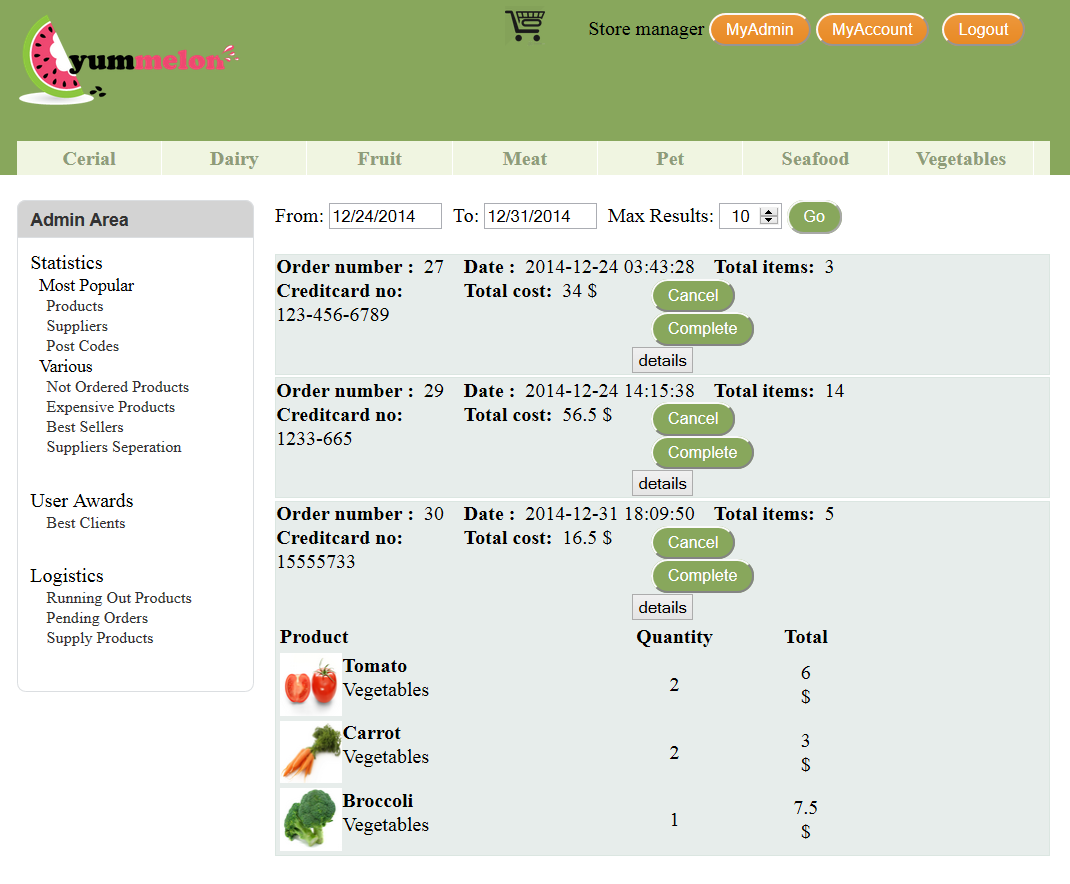
\includegraphics[width=1\textwidth]{pendingOrders}
				\caption{Εν'εξελίξει παραγγελείες}
			\end{figure}
			\begin{figure}[H]
				\centering
				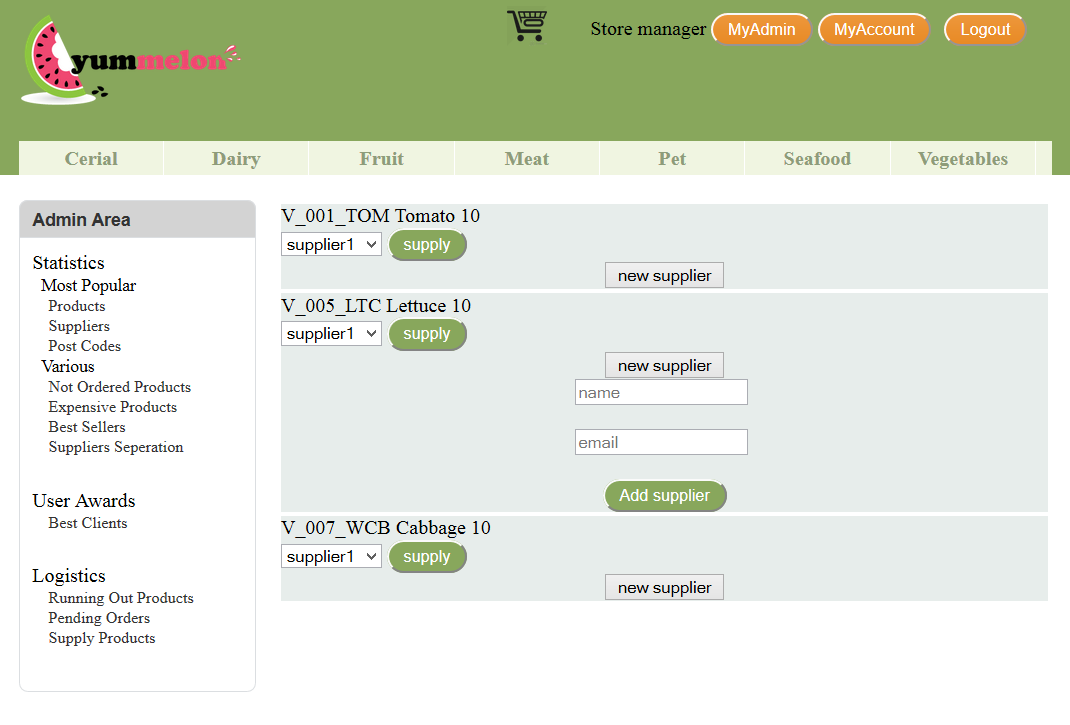
\includegraphics[width=1\textwidth]{supplyProducts}
				\caption{Προμήθευση προιόντων}
			\end{figure}	  

\end{document}